\chapter{Introduction au domaine}

\section{ Les architectures ARM }

Les architectures ARM sont introduites en 1983 et elles basés sur des architectures RISC (Reduced Instruction Set Computer) 32 bits (ARMv3 à ARMv7) et récemment 64 bits avec l'ARMv8.

\subsection{ Reduced Instruction Set Computer }

L'architecture RISC est un type d'architecture matérielle de microprocesseur. Elle est caractérisée par un jeu d'instructions réduit, facile à décoder et comportant uniquement des instructions simples. Elle s'oppose à l'architecture CISC (Complex Instruction Set Computer).
\\
Cette architecture est caractérisée par le fait de reposer l'optimisation du code sur le compilateur tandis que les instructions sont faciles à décoder pour le processeur. Pour cela :
\begin{itemize}
\item Ces processeurs possèdent un nombre important de registre "généraux" (un minimum de 16 et généralement de 32). Ils sont tous équivalents afin de faciliter leur allocation par le compilateur
\item Les instructions possèdent un taille fixe, souvent de 32 bits
\item Les instructions utilisées pour des calcules arithmétiques possèdent généralement 3 adresses avec 2 registres comme opérandes et un registre de sortie
\item Pour les accès à la mémoire, des instructions spécifiques sont employées et une valeur doit, au préalable, être chargée dans un regsitre pour être utilisée. Ce genre d'architecture est nommé load-store ou instruction register-register
\end{itemize}
Afin d'améliorer les performances, des ajouts ont été effectuées. Par exemple des instructions plus petites ou des méthode de compression de code ont été ajoutés ou encore les fenêtres de registres qui permettent une accélération des appels de fonctions sur certaines architectures.
Les architectures actuelles ont aussi la possibilité d'utiliser des instructions vectorielles et une unité de calcul en virgule flottante. 

\subsubsection{ Les avantages }

Un des principaux avantages de ce type de processeurs est dut à la présence d'instruction simple. En effet, gràce à ce type d'instruction, l'exécution du processeur est rapide, idéalement en un seul cycle, voire deux instructions en un cycle. Par exemple, certains processeurs RISC présents sur des calculateurs plus puissants se sont vu ajouter des instructions de type MULADD (multiplication + addition). Ce type d'instruction est très utilisé pour des calcul vectoriel et matriciel. Cela avait pour effet, par exemple, de prendre un seule cycle pour multiplier deux registres, y ajouter un autre registre et sauvegarder le résultat dans l'un de ces registres ou dans un autre.\\
Un autre avantage consiste à la faible perdition thermique de ce type de processeur contrairement au architecture CISC. En effet, on constate une utilisation des processeurs ARM sur des appareils mobile sans un système de refroidissement lourd (ventilateur) à la différence d'un ordinateur équipé d'un processeur CISC.

\subsubsection{ Les inconvénients}

L'un des inconvénients est la faible lisibilité du code d'un programme en assembleur surtout lorsqu'une optimisation de celui-ci est nécessaire.
Le code RISC est aussi généralement moins compact car toutes les instructions sont de même taille au contraire des instructions CISC qui sont généralement plus courtes.  


Cela se paye au prix d'une certaine diminution de lisibilité du code gênante lorsque l'on programme en assembleur et surtout si on l'optimise : l'instruction MVC (MoVe Character) du Système 360 restait tout de même plus lisible que la séquence d'instructions faisant la même chose dans une machine RISC. Mais pour qui codait strcpy() en langage C, il n'y avait plus aucune différence. Et en temps d'exécution, le code C optimisé se montrait en général plus performant en vitesse pure grâce à des astuces d'usage de l'effet pipeline par le compilateur.
Le code RISC est généralement moins compact, puisque toutes les instructions sont de même taille, alors que les instructions les plus utilisées sont plus courtes dans un jeu d'instruction CISC.

\subsection{ SoC (System on Chip) }

Un System on Chip ou SoC est une puce intégrant un microprocesseur, processeur graphique, d'autre fonctionnalité et contrôleur de périphériques. Ce type de système se retrouve sur à la majorité des tablettes et smartphones. ARM propose des architectures différentes selon le SoC employé. Chacun des constructeurs exploitant l'ARM peut ainsi ajouter des options propres ou de concepteurs tiers à leur architecture. Ainsi on a vu apparaitre, pour les socles d'aujourd'hui, les microprocesseurs Cortex, l'Apple A6 par exemple composé de technologie du cortex-A9 et cortex-A15 ou encore le TEGRA produit par Nvidia ayant une orientation plus vers la capacité graphique.

\begin{figure}[h!]
\begin{center}
	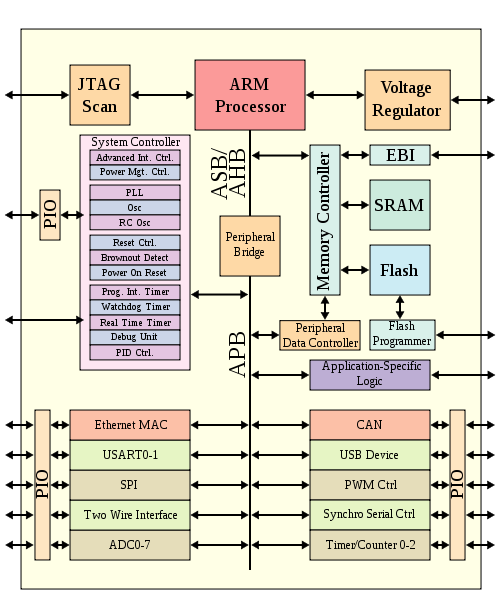
\includegraphics[scale=0.9]{ARMSoCBlockDiagram.png}
	\caption{Exemple de SoC}
\end{center}
\end{figure}

\subsection{ NEON }

NEON correspond au SSE pour les processeurs ARM. (A compléter)


\clearpage

\section{ Architecture x86 et x86-64 }

L'architecture x86(32 bits) x86-64(64 bits) est l'architecture la plus utilisée sur les ordinateurs aujourd'hui. Elle utilise les jeu d'instruction de type CISC (Complex instruction set computer). On observe par contre une absence de ce type d'architecture sur les appareils nomades. 

\subsection{ Complex instruction set computer }

Les microprocesseurs à jeu d'instruction du type CISC utilisent de très nombreuses instructions mixées à des mode d'adressages complexes. 

\subsubsection{ Avantage }

Ce type de jeu d'instruction possèdent plusieurs avantages :
\begin{itemize}
	\item L'empreinte mémoire du code est beaucoup plus dense. Par exemple on observe un facteur deux entre de l'ARM thumb et le x86). Cela pour effet de permettre l'utilisation minimal de la taille du cache instruction.
	\item Elle permet aussi de la microprogrammation, donc de corriger le jeu d'instructions. Cela facilite la correction de bug.
	\item Avec l'architecture CISC, on peut utiliser des instructions plus complexe non ou mal gérées par les compilateurs mais très rapide.
\end{itemize}

\subsubsection{ Inconvénient }

Ce type de microprocesseurs est plus difficile à accélérer. Leur structure est généralement plus complexe que sur une architecture RISC.





Le microprocesseur est plus compliqué à accélérer (problème pour pipeliner le moteur d'exécution).
Le processeur est globalement plus complexe qu'un processeur RISC.
Les compilateurs ont des difficultés à générer des instructions complexes.
Certaines instructions complexes sont exécutées sur plusieurs cycles d'horloge, dont le nombre peut dépendre des arguments. Il est difficile de prévoir la durée de certains calculs, ce qui peut mener à des problèmes de synchronisation.

 



